
\section{Fonti dei dati, indicatori sanitari, sorveglianza}

\subsection{Cronaca}


La Gazzetta di Parma del 05/10/2016 riporta 3 notizie legate alla Sanità
Pubblica:

\begin{enumerate}
\def\labelenumi{\arabic{enumi}.}
\item
  La seconda vittima di Legionella e il 31esimo caso, siamo di fronte ad
  un'epidemia
\item
  Capitolo ambiente, gestione dei rifiuti
\item
  La modifica costituzionale include anche cambiamenti per quanto
  riguarda la materia sanitaria (verrà trattata nelle lezioni di
  organizzazione sanitaria); vengono riportate allo stato alcune
  competenze legislative che erano state date nel 2001 alle regioni,
  quindi, se il referendum verrà approvato, dal punto di vista della
  struttura del sistema sanitario ci saranno più decisioni al centro e
  meno nelle regioni
\end{enumerate}

L'epidemia in corso riguarda la Legionella, un batterio ambientale, non
c'è trasmissione interumana dimostrata, c'è contaminazione ambientale in
vario modo: soprattutto immissione di aria o di aerosol nell'ambiente.
Gli ultimi focolai epidemici hanno riguardato condutture idriche o
impianti di distribuzione dell'aria.

Com'è stata scoperta la legionellosi 40 anni fa? È stata scoperta perchè
ci fu una riunione a Philadelphia di veterani del Vietnam che si
ritrovano annualmente cercando alberghi non utilizzati, fuori dalle
stagioni turistiche per spendere poco. Questi alberghi venivano riaperti
per queste convention e la Legionella, se viene lasciata nei filtri
d'aria, non ben mantenuti, presenti negli impianti di climatizzazione,
si moltiplica e alla riaccensione degli impianti viene immessa in
quantità importante nell'aria. Ciò ha portato ad un'epidemia. Inoltre i
veterani avevano una certa età, e quindi ci fu il primo caso epidemico
di Legionella che da quel momento in poi fu battezzata ``la malattia dei
legionari''.

La legionella è un batterio ambientale che, se presente in basse
concentrazioni non porta grandi rischi, a meno che ci sia una
suscettibilità dell'ospite (secondo elemento che nell'attuale epidemia è
fondamentale). Quindi, c'è una fonte d'immissione, probabilmente nel
caso di Parma sono le condutture idriche. Nelle condutture idriche poco
utilizzate, con incrostazioni, la Legionella c'è, si moltiplica in un
range di temperatura che va dai 20 ai 40C; si tratta di condutture in
stagione estiva o condutture dove passa l'acqua calda e quindi le
Legionelle vengono immesse nell'aria alla riapertura delle condutture
come aerosol e vengono respirate. A volte possono esserci microepidemie
nelle strutture ospedaliere. La legionella è termolabile, per cui con
l'acqua a 60C c'è l'inattivazione, come per l'acqua a temperature
minori.

Una precauzione individuale è quella di lasciar un po' scorrere l'acqua
prima di lavarsi la faccia, perchè altrimenti viene respirato l'aerosol
del primo getto; ciò riguarda soprattutto impianti usati poco, perchè se
sono impianti usati molto il problema non si pone. Se lo respira un
soggetto giovane immunocompetente non gli succede nulla, ha una forma
asintomatica; ma se lo respira un immunodepresso o un anziano può dare
molti problemi. A Parma non è ancora stata identificata esattamente la
fonte di partenza.

Quando ci sono i morti la psicosi epidemica ha sempre un forte impatto.

\subsection{Fonti dei dati}


Gli argomenti del primo parziale, sono 2: Metodologia epidemiologica,
Profilassi delle malattie infettive. Verranno trattatati fino all'ultimo
Venerdì di Ottobre, in totale dovrebbero essere 11 lezioni.

\subsubsection{Epidemiologia}


\begin{itemize}
\item
  Deriva dal greco ``studio sul popolo''
\item
  Scienza che studia le malattie e i fenomeni ad essere correlati a
  livello di popolazione
\item
  Include studi sulla frequenza delle malattie, sui fattori di rischio,
  sui servizi sanitari
\end{itemize}

L'epidemiologia nasce come disciplina che studia le epidemie delle
malattie infettive: Colera (Londra, 1870). Nasce per studiare le
malattie infettive, ma in un secondo tempo con gli stessi metodi si sono
studiate le malattie non infettive, i fattori di rischio e i
bisogni/servizi sanitari.

Siamo abituati a considerare l'epidemiologia uno strumento e non una
disciplina: è uno strumento che si applica spesso alla sanità pubblica e
alla medicina clinica.

Queste lezioni hanno lo scopo di farci comprendere le principali
tecniche epidemiologiche che possono essere usate in sanità pubblica, ma
anche nelle varie discipline/specialità con qualche aggiustamento e
particolarità.

Esempio 1. L'epidemiologia psichiatrica ha come punto debole del
meccanismo di valutazione il fatto che le diagnosi sono variopinte e non
sempre riconducibili a delle situazioni oggettive.

Esempio 2. L'epidemiologia dei tumori ha a che fare con dei dati molto
più oggettivi, però chiede di occuparsi dei fattori di rischio (non
sempre facilmente analizzabili).

C'è una parte dell'epidemiologia (clinica) applicata alle
sperimentazioni dei nuovi farmaci/trattamenti ed è quello strumento che,
insieme alla statistica, consente di poter fare le sperimentazioni e di
poter dimostrare, dove possibile, che nuovi trattamenti sono migliori di
quelli descritti.

Quindi abbiamo a che fare con uno strumento di lavoro che, come tale,
deve basarsi su dati.

L'epidemiologia analizza dati. In 2 modi l'epidemiologia si occupa di
dati:

\begin{enumerate}
\def\labelenumi{\arabic{enumi}.}
\item
  \textbf{approccio DESCRITTIVO}: descrive i fenomeni sanitari.
\end{enumerate}

\begin{quote}
Prende dati esistenti, già presenti e raccolti attraverso le fonti, li
riordina/analizza/stratifica e produce le statistiche sanitarie. Magari
con qualche correlazione tra l'andamento di un fenomeno e condizioni
esterne, ambientali, sociali, economiche; ma tendenzialmente descrive il
fenomeno. Difficilmente con la descrizione dei fenomeni si riesce ad
arrivare all'identificazione delle cause che, invece, attiene alla parte
dell'epidemiologia analitica.
\end{quote}

\begin{enumerate}
\def\labelenumi{\arabic{enumi}.}
\item
  \textbf{approccio ANALITICO}: indagare le cause / i determinanti.
\end{enumerate}

\begin{quote}
Accanto ai dati esistenti si cercano dati oggettivi per poter associare
la malattia ai fattori di rischio. Es. per scoprire la causa della
Legionella bisogna vedere caso per caso, vedere dove vivono, che
abitudini hanno le persone, se sono state o meno esposte a certi fattori
di rischio che potrebbero esser quelli ad aver causato la sua
diffusione.
\end{quote}

Quindi, l'epidemiologia descrittiva elenca i casi, l'analitica va a
cercare le cause e non sempre ci riesce.

Per soddisfare il primo obiettivo, i dati spesso ci sono, anche se non
sempre sono attendibili al 100\%. A volte sono disponibili ed
utilizzabili immediatamente, a volte sono parzialmente disponibili
(ossia sono raccolti ma devono essere elaborati), altre volte non ci
sono (bisognerà fare indagini ad hoc per cercarli).

\paragraph{Fonte di dati epidemiologici}


\begin{itemize}
\item
  Dati disponibili
\item
  Dati parzialmente disponibili
\item
  Dati non disponibili
\item
  Finalità sanitaria
\item
  Finalità amministrativa
\item
  Finalità di ricerca
\item
  Dati aggregati
\item
  Dati individuali
\end{itemize}

Esempio di \textbf{dati sanitari disponibili} (aprendo il computer e
cercandoli): schede di dimissione ospedaliera e report sulle cause di
ricoveri in Italia. A livello centrale si raccolgono i dati sui ricoveri
che hanno un duplice significato: finalità sanitaria, ma soprattutto una
finalità amministrativa.

Le schede di dimissione ospedaliera:

\begin{enumerate}
\def\labelenumi{\alph{enumi})}
\item
  sono fatte per tutti i pazienti dimessi
\item
  tendono a riportare le diagnosi di dimissione in maniera abbastanza
  precisa, perchè da quello dipende il rimborso alla struttura
  ospedaliera per la prestazione erogata
\item
  devono essere attendibili, perchè soggette a controlli
\end{enumerate}

Esempio di \textbf{dati sanitari parzialmente disponibili}: cartelle
cliniche (i dati ci sono ma non sono raccolti e rielaborati). Se voglio
fare una ricerca per una determinata malattia: prendo, con tutti i
permessi e i nulla osta dei comitati etici, le cartelle cliniche,
raccolgo e ricopio tutti i dati che a noi interessano.

Esempio di \textbf{dati sanitari non disponibili} (non c'è nessuna fonte
che li raccoglie). È il gruppo più numeroso. Se volessi sapere quanti
sono i fumatori in Italia i dati non li troverei. Non c'è un elenco
nazione dei fumatori, come non c'è l'obbligo di dichiarare le proprie
generalità all'acquisto di tabacchi. Non ho i dati, ma posso stimarli in
2 modi: prendendo il dato del Monopolio di Stato che ci dice quanti
pacchetti di sigarette sono venduti, questo è un dato che può monitorare
il trend degli anni oppure facendo un'indagine a campione (telefonate a
casa o questionari).

Quindi, quando studio un problema, devo sempre chiedermi se i dati ci
sono o meno.

Ci sono situazioni in cui posso cercare di prendere i dati ma questi non
sono attendibili: più delicato è il tema, più difficile è la raccolta
del dato, soprattutto sulle abitudini individuali.

Es. Se volessi analizzare quante sono le lesioni da morsicatura di cane.
Negli USA muoiono ogni anno 20 persone morsicate da un cane, in Italia
ne muoiono 3-4. Nelle schede dei pronti soccorsi troviamo quanti
pazienti entrano con la diagnosi di morsicatura di animale e i dati sul
ricovero se la lesione è grave. Non ho modo di trovare dati che
riguardano le medicazioni ambulatoriali o le automedicazioni, devo fare
delle stime, ma a volte l'indagine campionaria può non essere
attendibile spesso perché i soggetti coinvolti non ricordano. Un'altra
grande difficoltà si ha nelle indagini nutrizionali, se chiedo ad un
campione di persone di raccontarmi ciò che ha mangiato nell'ultimo anno
e qual è il pasto medio, è possibile che non si ricordino e quindi non
forniscono un dato attendibile.

Il dato deve essere sempre pesato in relazione alla sua attendibilità.

Ho dati di attendibilità piena, come la scheda di morte che è un dato
oggettivo, sempre presente; sulle cause di morte i dati sono meno
attendibili, perchè ci può essere qualche notifica non precisa.

Tra i dati disponibili: schede di morte, schede di nascita, notifica
delle malattie infettive, schede di dimissione ospedaliera, cartelle
cliniche. Oltre a questa fonte di dati prettamente sanitari, abbiamo
dati più demografici/economici come il censimento che raccoglie dati
demografici, economici, sugli ambienti di vita, sulla mobilità.


\begin{figure}[!ht]
\centering
	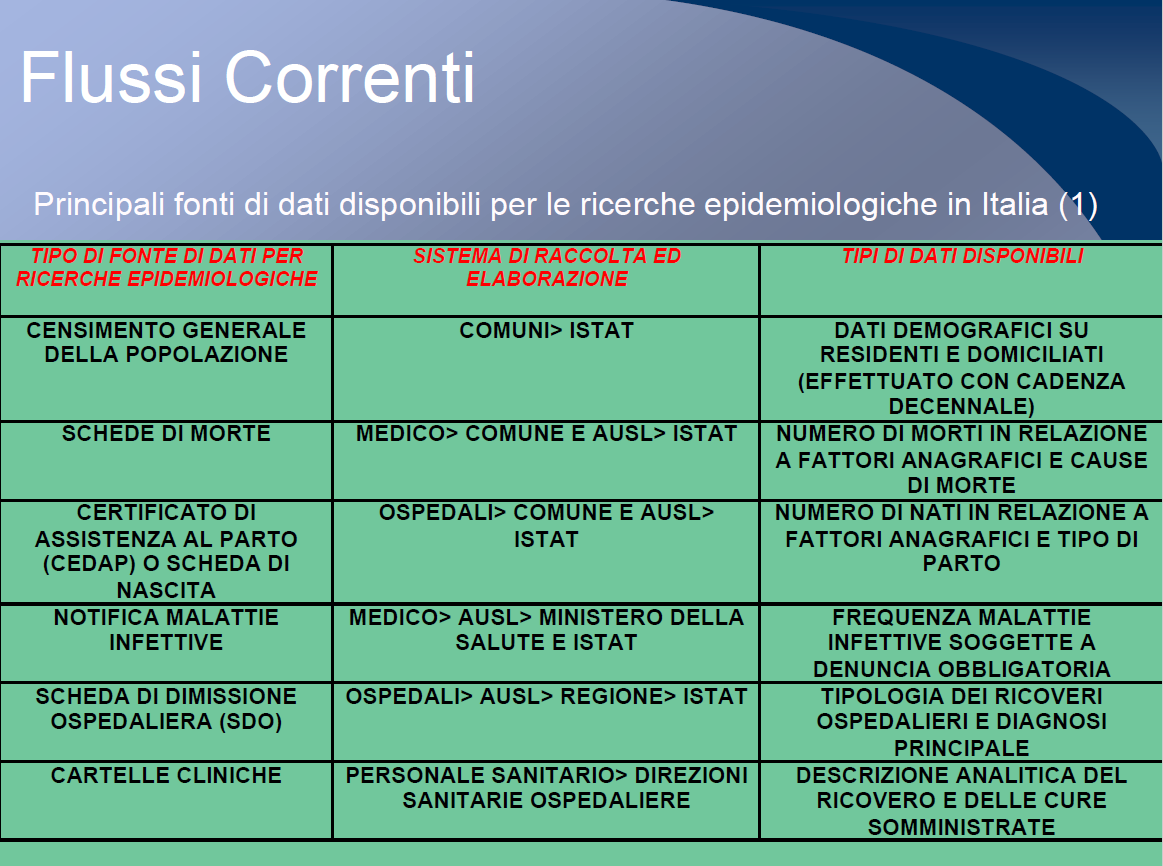
\includegraphics[width=0.9\textwidth]{02/image1.png}
\end{figure}



\paragraph{Notifica delle malattie infettive}

La notifica delle malattie infettive merita una segnalazione. Ogni tanto
c'è qualche caso di Legionella, oggi a Parma c'è un episodio epidemico;
ma i casi di Legionellosi comunque ci sono. Se sono lievi la probabilità
che questi casi vengano notificati non è altissima, cioè il medico
potrebbe, se i sintomi sono generici e aspecifici, non chiedere indagini
diagnostiche e quindi quel caso non è notificato oppure il medico
potrebbe, anche in presenza di accertamento diagnostico, non notificare
perchè il paziente viene visitato in ambulatorio dove i tassi di
notifica sono meno stringenti rispetto alla struttura ospedaliera.
Quindi noi siamo certi che tutte le Legionellosi che arrivano in
ospedale vengano notificate, ma non ne siamo affatto certi per le
Legionellosi che arrivano in ambulatorio.

La notifica delle malattie infettive risente della sottonotifica, questa
è tanto maggiore quanto di minor gravità è la malattia. Se leggo sulle
statistiche che ci sono 1000 casi di malaria all' anno, ritengo che
questo dato sia molto attendibile; perchè la malaria è una malattia che
quando viene vista viene notificata.

Quando trovo 1000 casi di morbillo, non sono convinto che questi siano
in realtà tutti casi di morbillo; perchè abbiamo a che fare con una
malattia che nella maggior parte dei casi è di lieve impatto e non
sempre viene notificata: vengono notificati circa 2 casi su 10 di
morbillo, quindi abbiamo il 20-30\% di tasso di notifica.

Quando ci sono le epidemie, i medici diventano scrupolosissimi, quindi
dei 31 casi di Legionellosi a Parma siamo certi, perchè oggi qualunque
caso di sospetta Legionellosi richiede l'accertamento diagnostico.
Quindi l'episodio epidemico tende a rende il medico più scrupoloso nella
diagnosi e nella notifica del caso. Dunque, anche la stessa fonte, in
momenti diversi, può essere più o meno attendibile.


\begin{figure}[!ht]
\centering
	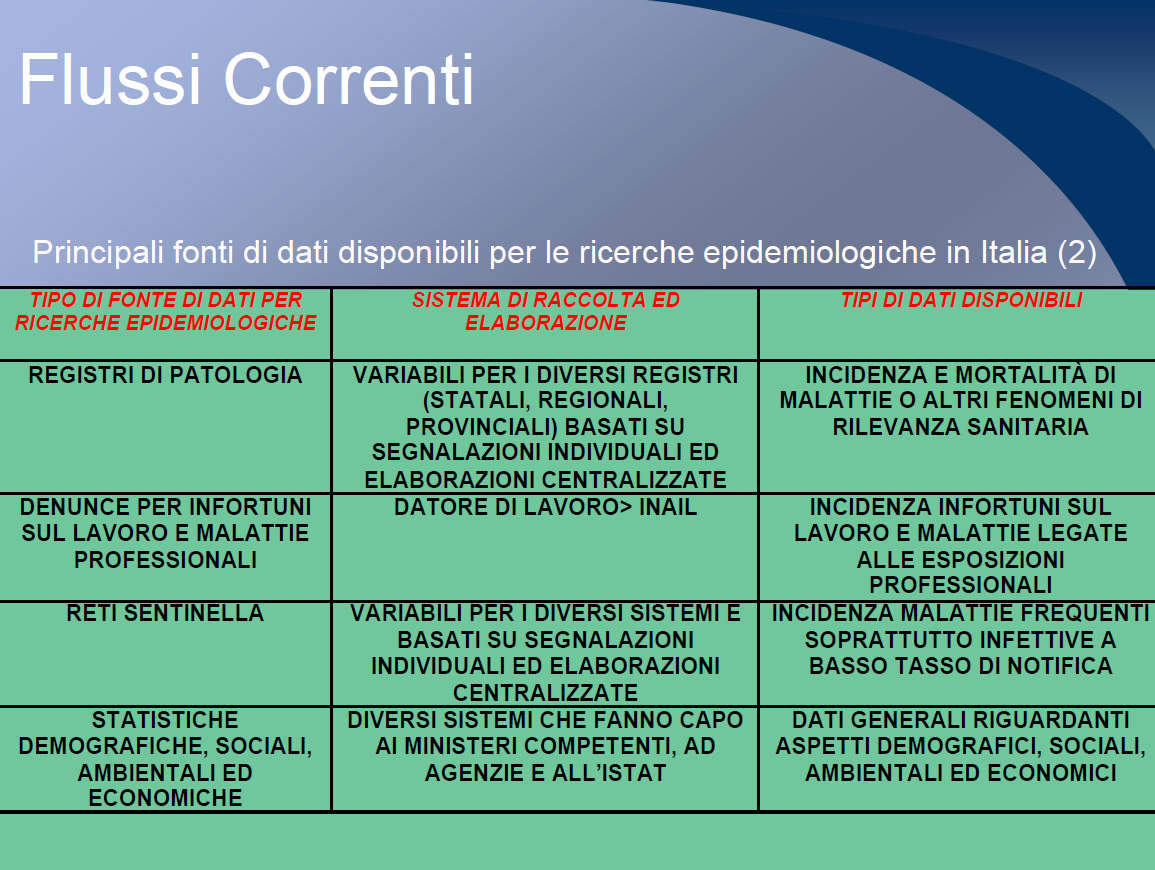
\includegraphics[width=0.9\textwidth]{02/image2.png}
\end{figure}


\paragraph{Registri di patologia}


Es. registro dei tumori (c'è a Parma e in altre 15 province italiane).

Al contrario delle malattie infettive, noi non abbiamo l'obbligo di
notifica dei tumori, però il paziente col tumore, durante la sua
malattia (solitamente nelle prime fasi) va in ospedale, quasi tutti i
tumori maligni accedono ad una struttura ospedaliera, quindi avranno la
loro SDO e questa avrà una diagnosi che riporterà quel tumore, se
confermato da accertamenti diagnostici.

Se vado a leggere quanti ricoveri per tumore al polmone ho in un anno
tra i residenti nella provincia di Parma e scopro che sono 2500 ricoveri
con diagnosi di tumore al polmone, questo dato mi serve ai fini di
valutare il numero di tumori o i nuovi casi di tumore? No. Da
epidemiologo mi serve sapere quanti sono i nuovi casi, quanti sono i
casi presenti e sapere come negli anni va la malattia. Quindi questo
dato non mi basta, perchè i 2500 potrebbero essere tutte persone che
entrano una volta, ma anche meno persone che vengono ricoverate più
volte, alcuni di questi potrebbero già avere il tumore e rientrare in
ospedale per una complicazione o una cura, altri sono nuovi casi. In
realtà i dati ci sono ma occorre riordinarli per poter calcolare
l'incidenza della malattia.

Il registro tumori raccoglie tutti i dati diagnostici incrociandoli con
i dati anagrafici e compone un quadro per tutti i tumori maligni di
numero di nuovi casi, incrociandoli con le schede di morte di questi
pazienti, si riesce anche ad avere il dato di mortalità e anche di
letalità dei tumori (i dati di sopravvivenza dalla prima diagnosi). Il
registro tumori dà dei risultati attendibili. Il presupposto
fondamentale è che ci sia l'accesso al sistema ospedaliero di tutti i
tumori, è quasi vero, perchè perdiamo qualche paziente che si cura in
strutture private o all'estero (questi casi non vengono visti dalle
statistiche). Le SDO sono compilate dalle strutture pubbliche e dalle
strutture private accreditate di tutta Italia, quindi è possibile con
agilità ricostruire i dati dei cittadini di Parma che vanno a farsi
curare in tutta Italia, perchè la SDO arriva all'ASL per il pagamento
della prestazione. Però in Italia l'accesso delle strutture private
pure, è marginale per malattie di questo tipo (tumori).

Si tratta di dati che non potrei avere in nessuna delle altre fonti,
nella scheda di morte c'è la causa di morte, ma non tutti i tumori sono
ad alta letalità e qualcuno guarisce anche; quindi dal punto di vista
epidemiologico non sono soddisfatto dal dato di mortalità, lo potrei
essere per i tumori ad alta letalità, ma fortunatamente oggi molti
tumori non hanno una letalità altissima. Quindi per avere i dati
d'incidenza devo avere il registro dei tumori.

\paragraph{Reti sentinella}


Ci sono situazioni dove la malattia non è cosi grave da determinare il
ricovero ospedaliero, dove le notifiche non sono fatte bene, dove non si
muore o si muore molto poco. Un caso emblematico è l'influenza
(\textbf{sindrome} \textbf{influenzale}): si muore raramente, non si va
in ospedale se non per fatti gravi. In questi casi esiste una rete
sentinella in cui un campione ormai consolidato di medici di famiglia,
sparsi su tutto il territorio nazionale, fanno notifica attraverso un
sistema consolidato all'istituto superiore di sanità, secondo le linee
guida internazionali, ogni qual volta riscontrano sintomi riconducibili
all'influenza, secondo un protocollo che viene stabilito e con un certo
margine di errore/imprecisione che, però, è calcolato e può esser tenuto
in conto.

\begin{figure}[!ht]
\centering
	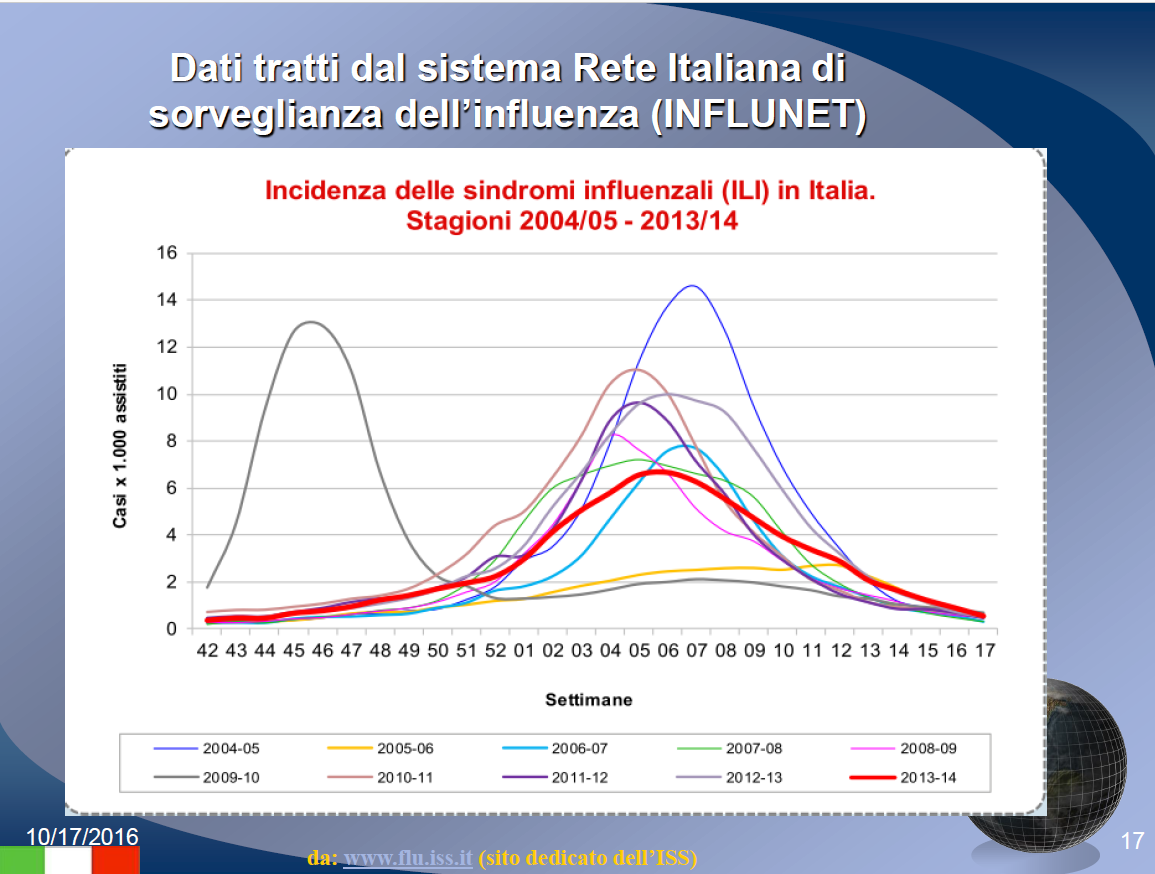
\includegraphics[width=0.9\textwidth]{02/image3.png}
\end{figure}


Ogni colore è una stagione invernale, anno per anno (per 10 anni) ci
disegna la frequenza delle sindromi influenzali in base alla settimana
dell'anno (1 -> 52). Cosa ci dice questo grafico?

Grossomodo, a prescindere dai picchi, in tutte le annate notiamo che
l'influenza comincia a diffondersi nelle ultime settimane dell'anno e
nelle prime 3-4 settimane del nuovo anno, quindi tra fine Dicembre ed
inizio di Gennaio e, termina a Marzo. Quindi la vaccinazione verrà fatta
entro l'inizio, ossia entro la metà di Dicembre.

Ci sono annate in cui il picco è più alto e altre in cui il picco è più
basso. Grossomodo nel decennio non notiamo un trend discendente o
ascendente. {[}Quando ci sono pochi cambiamenti antigenici, i soggetti
che hanno fatto la vaccinazione l'anno prima sono protetti, perchè c'è
la cross-reattività; ma quando arriva un virus nuovo i casi sono
maggiori.{]}

La curva grigia (anno 2009-2010) è l'anno in cui è arrivata la pandemia,
un nuovo virus con caratteristiche antigeniche completamente diverse,
con diversa distribuzione e il picco c'è stato a Novembre,
fortunatamente è stato un picco non acuto in termini di sintomi e di
gravità.

Dal punto di vista tecnico, con un grafico riesco a descrivere il
fenomeno in maniera molto chiara e molto semplice. L'epidemiologia ci da
anche qualche metodo per dimostrare i dati in maniera molto chiara. Una
raccolta di questo genere ci consente anche le differenziazioni per
fascia d'età.

Il sistema sentinella riporta il caso ma ne imposta anche le
caratteristiche.
\begin{figure}[!ht]
\centering
	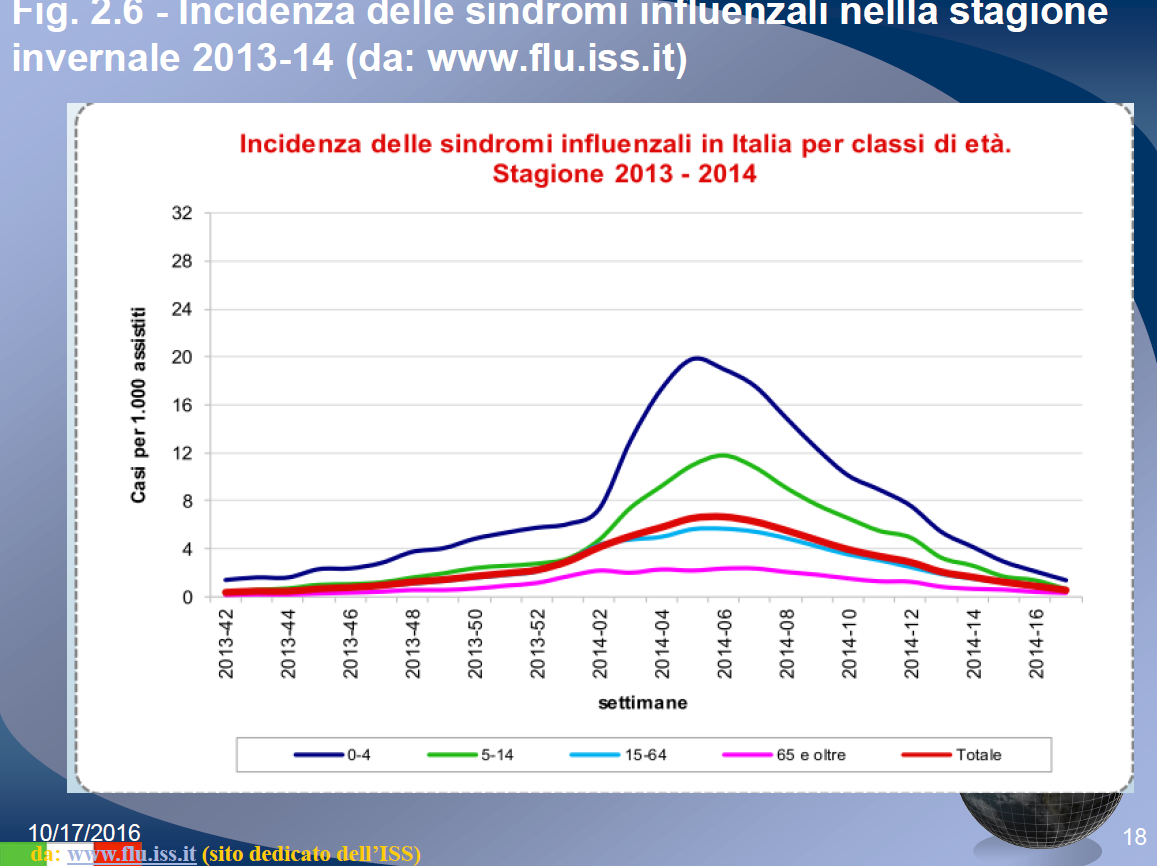
\includegraphics[width=0.9\textwidth]{02/image4.png}
\end{figure}


Distribuzione per un'annata (2013-2014) dei casi per fascia d'età. Si
nota che la fascia più colpita è quella infantile (0-4) seguita da
quella 5-14 anni.

Grazie ad una vaccinazione su larga scala fatta agli anziani,
l'influenza è più diffusa tra i bambini.

La vaccinazione si può fare nei bambini: negli USA è raccomandata a
tutti i bambini anche sani, in Italia è raccomandata solo ai bambini che
frequentano comunità affollate dove il rischio è maggiore.

\subsection{INDICATORI SANITARI}


Caratteristica di un individuo, di una popolazione o di un ambiente che
può essere quantificata ed è strettamente associata ad un fenomeno che
non è direttamente misurabile.

Es. Mortalità infantile \textgreater{} livello igienico

• Indicatori di sopravvivenza

• Indicatori dello stile di vita

• Indicatori di ``qualità di vita''

• Indicatori socio-economici

Indicatori sanitari, cosa sono? Gli indicatori sono dei dati, quasi
sempre epidemiologici, che misurano caratteristiche individuali o
collettive e che tendono a spiegare un fenomeno che non è direttamente
misurabile.

Se il fenomeno è lo stato di salute di una popolazione, devo trovare dei
dati che esemplifichino/quantifichino quel fenomeno che non è
direttamente misurato. Ho bisogno di dati oggettivi per misurare questo
stato di salute.

La \textbf{vita media} è un esempio di dato indicatore dello stato di
salute di una popolazione; se calcolo con le schede di morte che la vita
media della popolazione italiana è 81 anni, quella dell'Uganda è 55, c'è
in definitiva una bella differenza.

Quindi, l'indicatore sanitario misura un fenomeno.

L'indicatore non si ferma al dato sanitario. Ad es. c'è l'indicatore
economico che è il reddito medio della popolazione. Ogni dato va
contestualizzato e va valutata l'attendibilità.

La \textbf{mortalità infantile} è ancor più specifica della vita media
per valutare il livello igienico-sanitario di una popolazione. La
mortalità infantile è il numero di bambini morti nel primo anno di vita
diviso il numero di bambini nati vivi: alcune morti sono conseguenza di
malformazioni già presenti, altre sono legate a fattori ambientali; in
Italia è 5x1000, mediamente 5 bambini muoino nel primo anno di vita
rispetto a 1000 bambini nati vivi; nei paesi coi peggiori livelli
igienico-sanitari è 40x1000. Non sono considerate le morti fetali,
queste sono indicatori non dell'ambiente, ma dell'assistenza al parto.

\begin{figure}[!ht]
\centering
	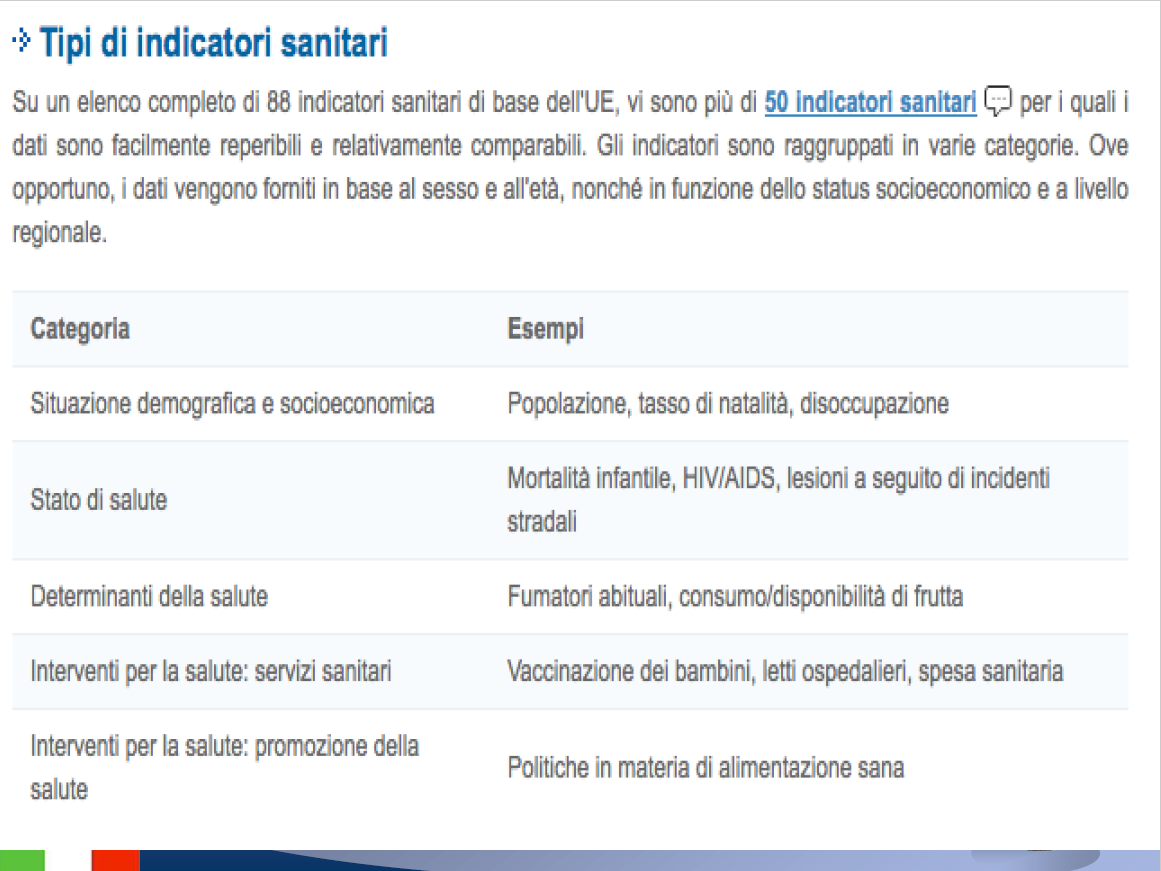
\includegraphics[width=0.9\textwidth]{02/image5.png}
\end{figure}


Abbiamo moltissimi indicatori sanitari su diversi ambiti; es. stato di
salute: mortalità infantile, incidenza di mortalità di AIDS, lesioni a
seguito di incidenti stradali. A seconda dell'obiettivo/studio/ricerca
possiamo prendere tutti i dati di cui abbiamo bisogno, usando le fonti
prima menzionate. Idem per i determinanti di salute, i fumatori, i
consumatori di alcool, percentuale di bambini vaccinati.

I dati abbondano, bisogna solo verificarne l'attendibilità, riordinarli
ed usarli per lo scopo della mia ricerca.
\begin{figure}[!ht]
\centering
	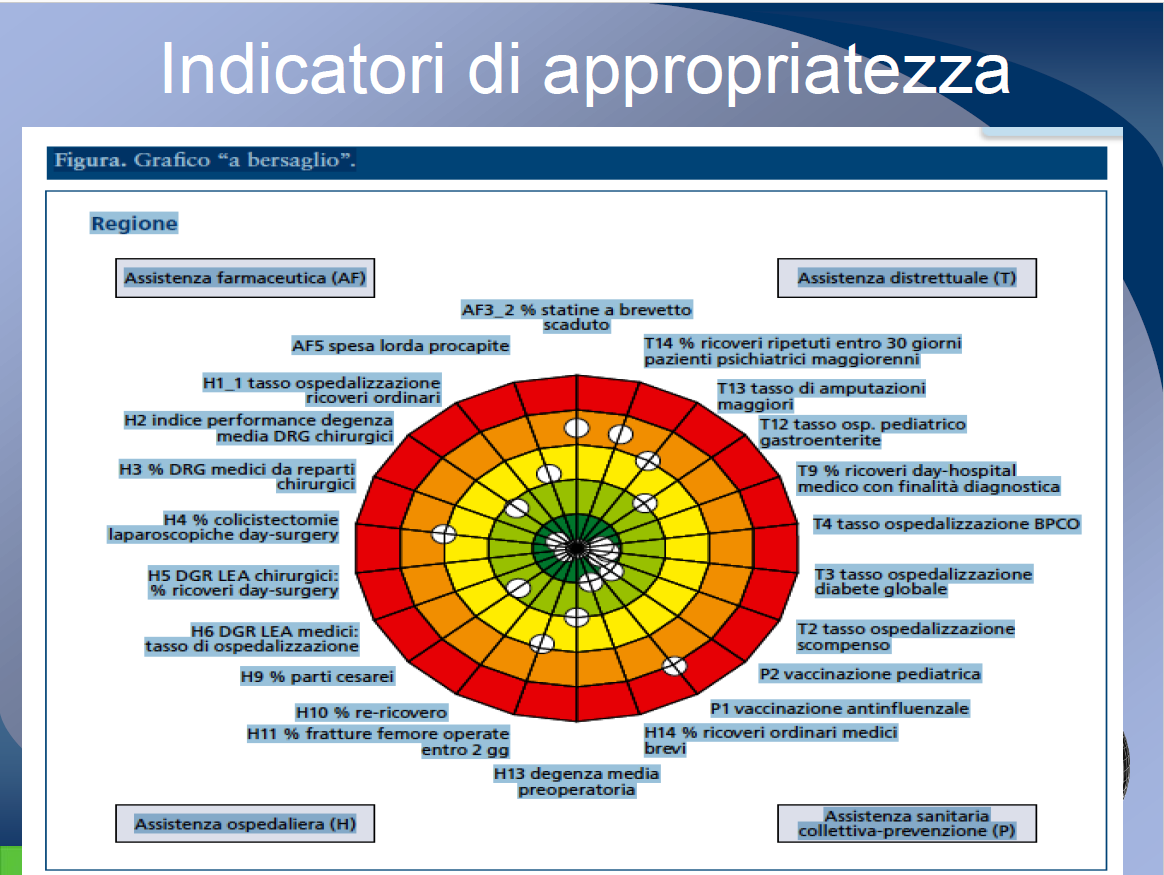
\includegraphics[width=0.9\textwidth]{02/image6.png}
\end{figure}


Trattamenti quali: degenza media pre-operatoria, frattura del femore
operato entro 2 giorni, \% dei parti cesarei, \% di colecistectomie
laparoscopiche in day surgery.

Sono tutti dati ed indicatori dell' assistenza sanitaria. Possiamo
vedere quali sono, regione per regione, le situazioni anomale rispetto
agli standard prestabiliti.

Qui non parliamo più di malattie, ma di assistenza sanitaria.
L'approccio è lo stesso.

\begin{figure}[!ht]
\centering
	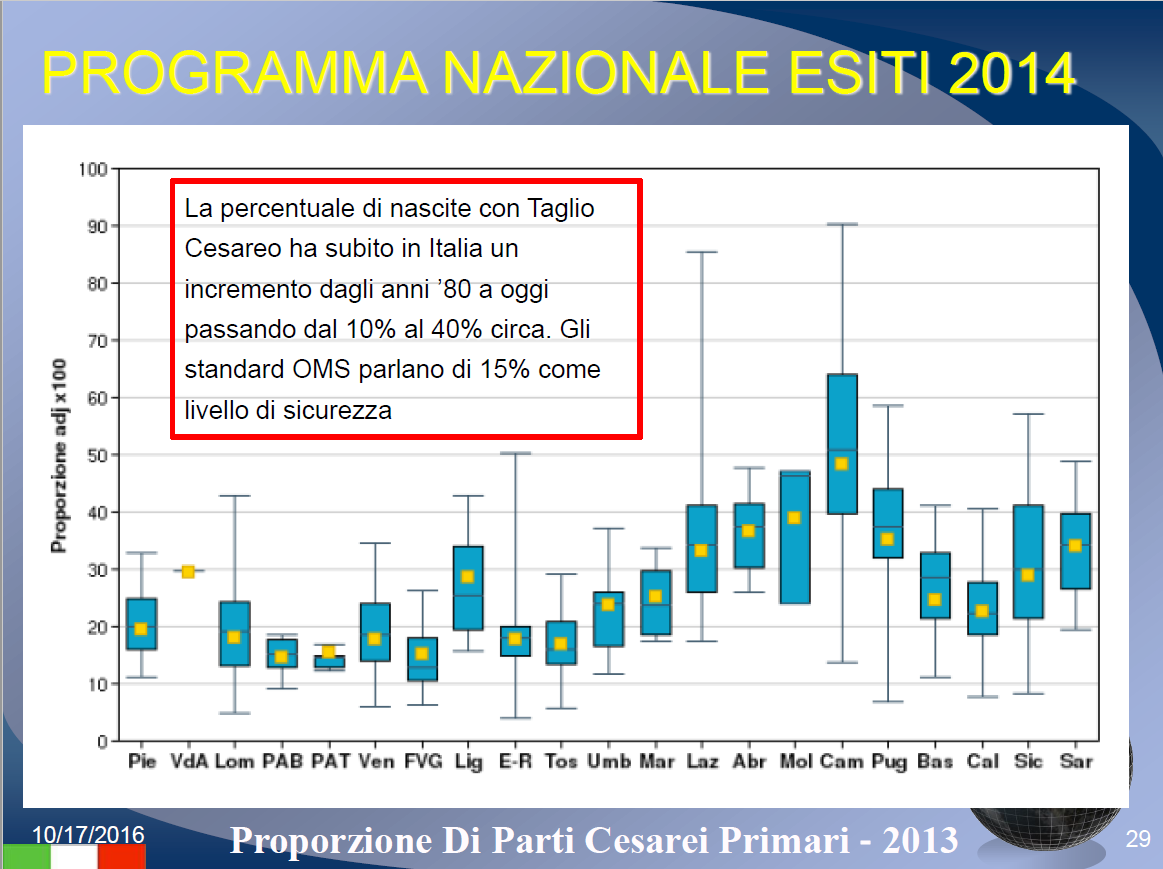
\includegraphics[width=0.9\textwidth]{02/image7.png}
\end{figure}


Queste sono le nascite con taglio cesareo nelle diverse regioni
italiane: un buon gruppo di regioni, soprattutto al Nord è sotto al
20\%, in altre regioni come la Campania si ha il 50\% di nascite con
taglio cesareo.

L'OMS ritiene che il 15\% di cesarei è sufficiente per far fronte a
quelle situazioni rischiose per la madre e per il feto. In Italia, negli
anni 80, la percentuale era del 10\%, ora siamo arrivati al 35\% ed è un
problema, perchè ciò comporta più costi e più complicazioni.

Ci sono una serie di motivi che lentamente hanno portato a questo
aumento di taglio cesareo, uno di questi è legato al non rischiare di
gestire dei parti complicati per via naturale preferendo la soluzione
del cesareo, perchè è più comodo, è più veloce e apparentemente più
sicuro (rischia meno il bambino, rischia più la madre). La mortalità
materna dopo taglio cesareo è 8 su 100.000; invece, la mortalità materna
dopo parto vaginale è 2 su 100.000. Ci sono 500.000 parti all'anno in
Italia, perdiamo almeno 30 donne morte dopo taglio cesareo: l'evento
accidentale è inevitabile dopo intervento chirurgico. Perchè succede
questo? Spesso è la partoriente a chiedere il parto con taglio cesareo,
firma e accetta il rischio; inoltre negli anni ci si è abituati a
gestire certe criticità col cesareo (presentazione podalica e parto
gemellare), si fa il cesareo e questa è diventata routine.

In Campania metà dei parti avvengono in strutture private non
accreditate, in tali strutture si va a prenotazione e si preferisce fare
un cesareo, perchè la durata è molto inferiore (30 minuti) rispetto al
parto per via vaginale (4-5 ore).

\subsection{Sistemi di sorveglianza sanitaria }

\begin{figure}[!ht]
\centering
	
\includegraphics[width=0.9\textwidth]{02/image8.png}
\end{figure}


Raccolta, attivazione, analisi dei dati seguiti dalla diffusione di
informazioni a tutte le persone potenzialmente interessate. Vi è una
sorveglianza di sanità pubblica, di luoghi di lavoro. La sorveglianza
sanitaria è un monitoraggio della situazione sanitaria con particolare
rilievo a qualche dato più importante, più sensibile di altro che
richiede interventi specifici e ad hoc.
\begin{figure}[!ht]
\centering
	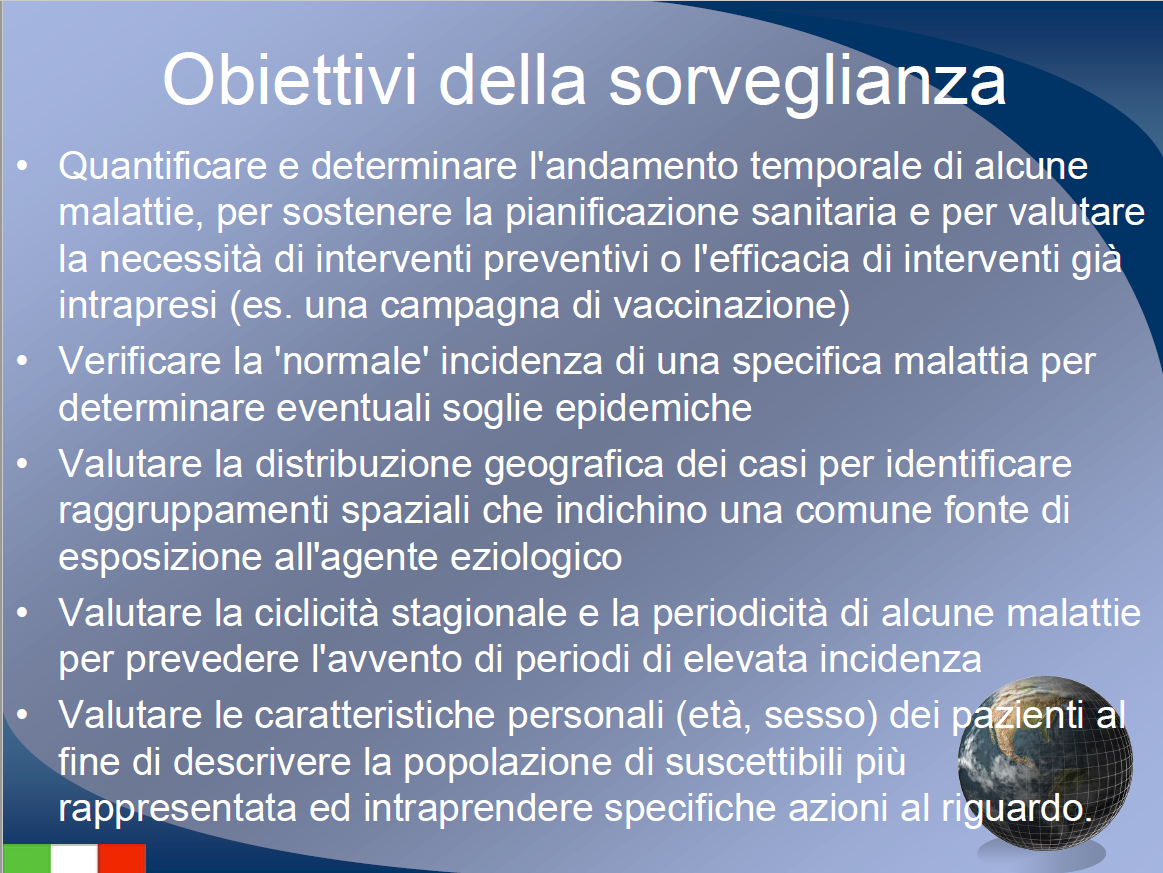
\includegraphics[width=0.9\textwidth]{02/image9.png}
\end{figure}


Obiettivi della sorveglianza: quantificare, determinare l'andamento
temporale di alcune malattie, verificare la normale incidenza,
verificare la distribuzione geografica, valutare la ciclicità
stagionale, valutare le caratteristiche personali. È una sorta di
``cruscotto'' che a livello locale, regionale, nazionale o
internazionale bisogna avere, perchè soprattutto per le patologie
infettive, dove sono più comuni i fenomeni epidemici, bisogna
intervenire laddove c'è un'anomalia notata in relazione al numero di
case. Le epidemie si identificano grazie alla sorveglianza sanitaria, se
non avessi il sistema delle notifiche non potrei dire che c'è in corso a
Parma l'epidemia di Legionellosi.
\begin{figure}[!ht]
\centering
	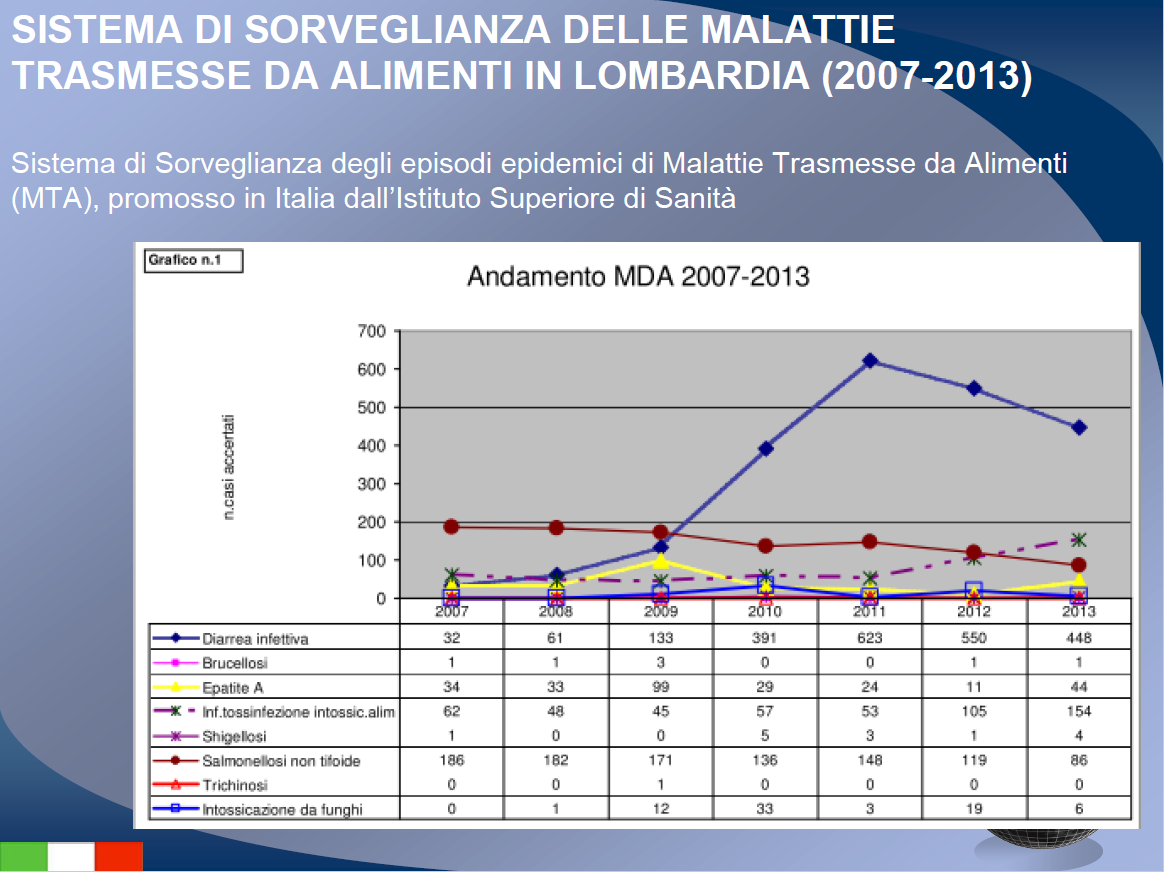
\includegraphics[width=0.9\textwidth]{02/image10.png}
\end{figure}


È un sistema di sorveglianza di malattie trasmesse da alimenti in
Lombardia: diarrea infettiva, brucellosi, epatite A, tossinfezione da
salmonella, trichinosi, intossicazione da funghi.

\begin{figure}[!ht]
\centering
	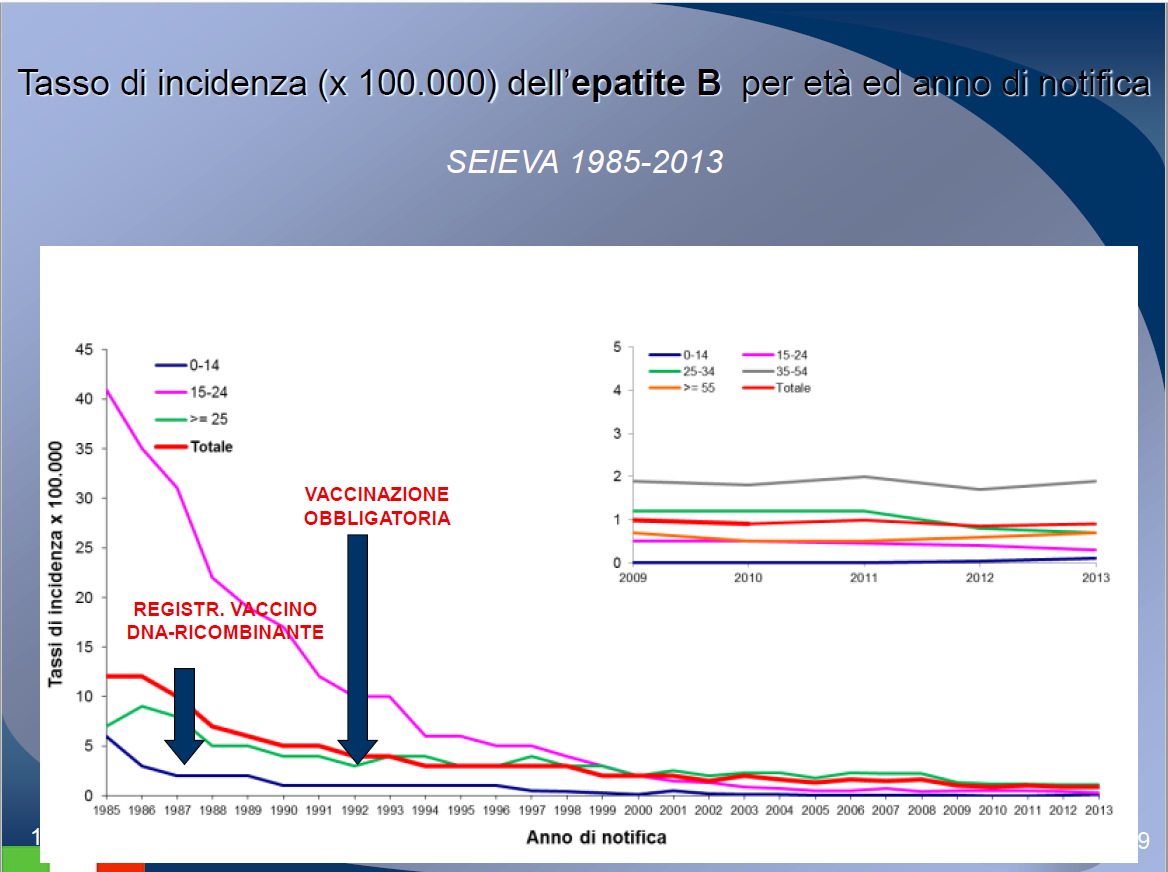
\includegraphics[width=0.9\textwidth]{02/image11.png}
\end{figure}


Sorveglianza dell'epatite B messa a punto dall'istituto superiore di
sanità. Questo grafico ci fa vedere che la malattia negli anni 80 già
scendeva, ma che è stato l'arrivo del primo vaccino nell'87 e del
vaccino obbligatorio nel 1992 che ha portato progressivamente ad una
diminuzione e quasi ad un azzeramento di casi.
\begin{figure}[!ht]
\centering
	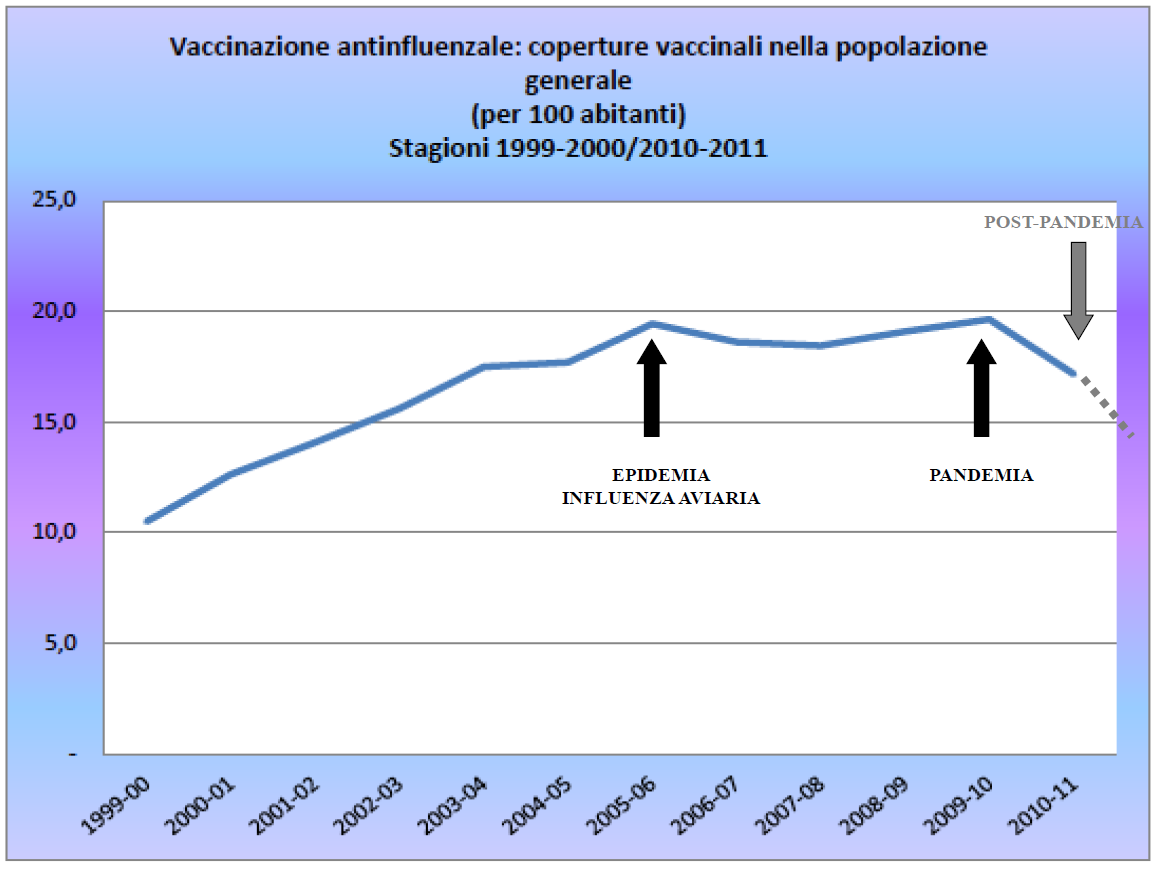
\includegraphics[width=0.9\textwidth]{02/image12.png}
\end{figure}


Andamento della vaccinazione antinfluenzale. Negli anni dell'epidemia
dell'influenza aviaria e nella pandemia c'è stata adesione più alta e
poi subito dopo dei cali di adesione alla vaccinazione.

Categorie raccomandate per la vaccinazione: malati cronici, ultra
65enni, bambini che frequentano comunità.

Gli operatori sanitari si vaccinano poco, non più del 15-20\%, questo è
un problema: in sé l'operatore sanitario non è un soggetto a rischio per
se stesso, ma può esser un rischio per i pazienti.
\begin{figure}[!ht]
\centering
	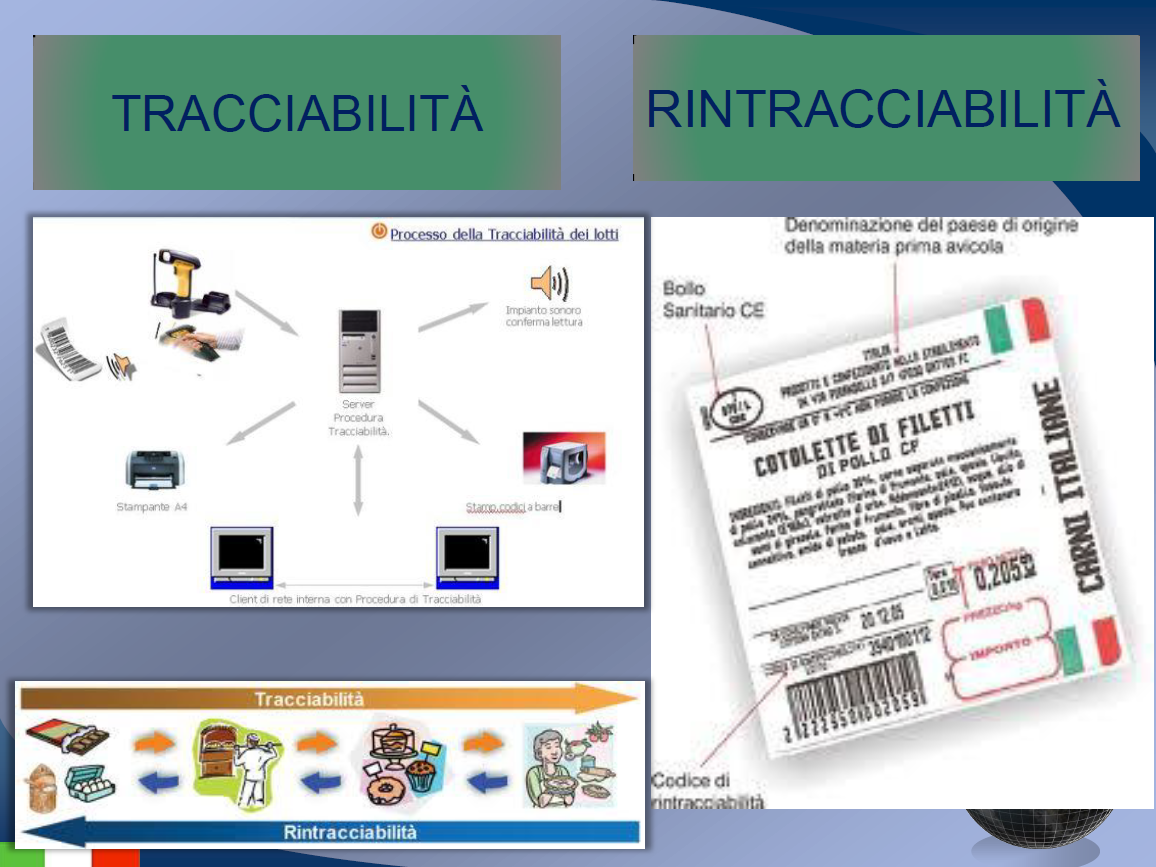
\includegraphics[width=0.9\textwidth]{02/image13.png}
\end{figure}


Sorveglianze per la tracciabilità alimentare con tutti i vari tipi di
controlli.

\begin{figure}[!ht]
\centering
	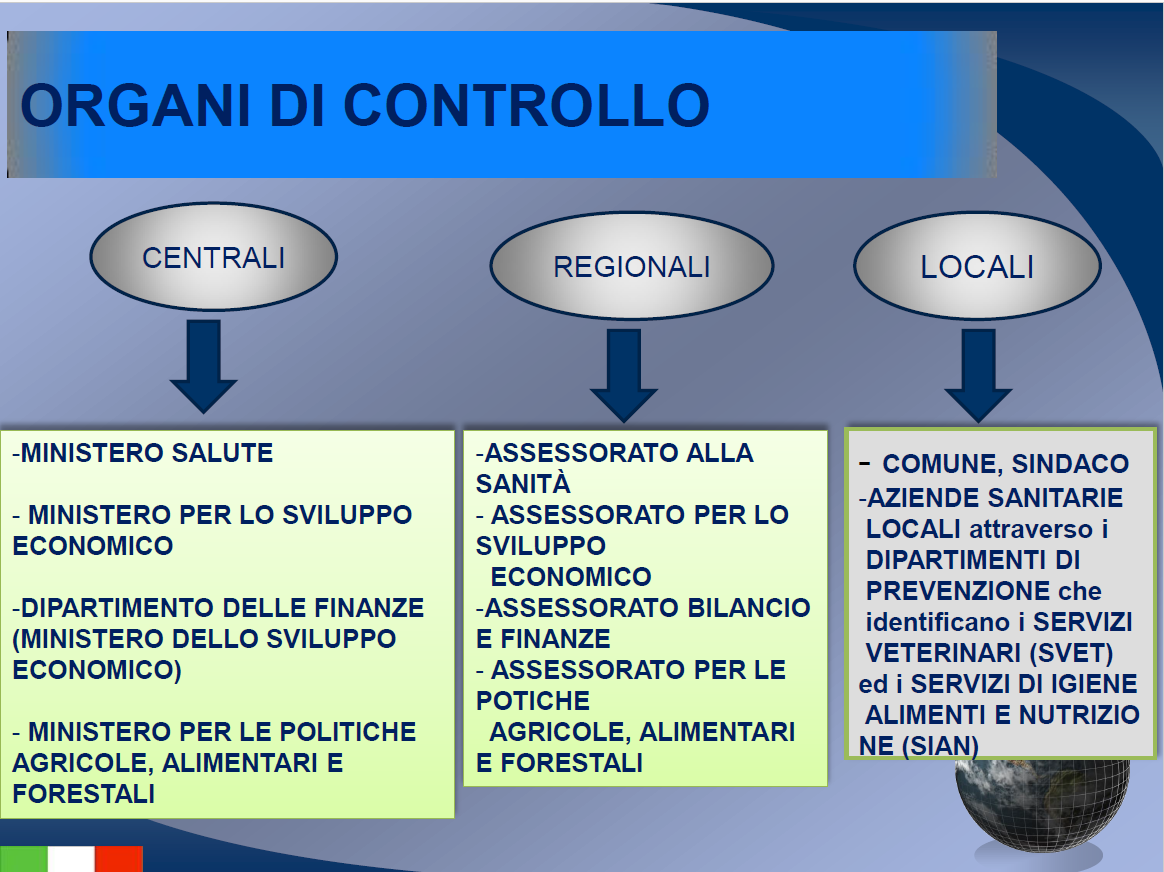
\includegraphics[width=0.9\textwidth]{02/image14.png}
\end{figure}


Il servizio sanitario nazionale non si occupa solo delle terapie e dei
ricoveri ospedalieri e in generale delle cure. Tutta questa filiera si
occupa dei controlli alimentari, questi sono un problema serio, in
Italia molto ben gestito che però mette in campo tutte queste strutture:
ministero della salute, ministero dello sviluppo economico, ministero
per le politiche agricole, forestale, alimentari, i vari assessorati
competenti nelle provincie e a livello locale; abbiamo da un lato le
aziende AUSL con i dipartimenti di prevenzione o i dipartimenti di
sanità pubblica, i servizi veterinari, i servizi di generi e alimenti
della nutrizione: tutti coinvolti nella filiera di verifiche, di
controlli a campione e di interventi in caso di problemi contingenti.

Qualche volta attivano i N.A.S. che sono un nucleo speciale dei
carabinieri specializzato nel settore sanitario, intervengono al bisogno
per ispezioni quando le autorità locali non ce la fanno o quando il caso
è talmente eclatante da dover indagare anche sulle mancanze
dell'autorità deputata al controllo, in questo caso si tratta di un
intervento ispettivo, è una anomalia, non è una routine. La routine
viene fatta attraverso questa filiera che parte dallo Stato e passa per
le regioni.
\begin{figure}[!ht]
\centering
	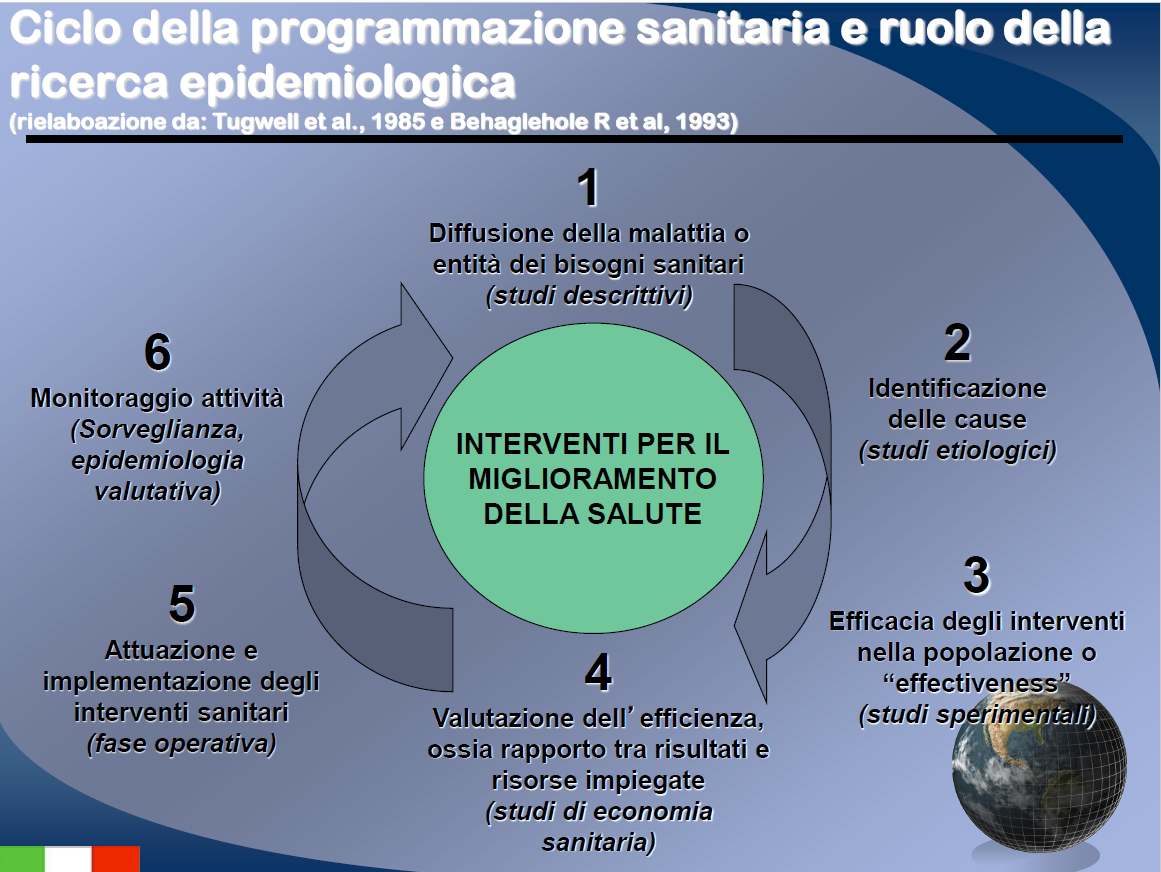
\includegraphics[width=0.9\textwidth]{02/image15.png}
\end{figure}


Questa diapositiva inquadra il ruolo dell'epidemiologia nella
programmazione sanitaria.

\textbf{1.} Per poter far bene la programmazione sanitaria bisogna
conoscere la situazione sanitaria e quindi bisogna conoscere la
distribuzione delle malattie e più specificamente quali sono i bisogni
sanitari di una popolazione che possono essere diversi tra una
popolazione e un'altra. In certi continenti abbiamo problemi sanitari
completamente diversi rispetto a quelli che abbiamo nel nostro paese. Se
facessimo programmazione sanitaria in Camerun e in tutti i paesi del
centro Africa ci dovremmo occupare in prima battuta di malaria,
HIV-AIDS, tubercolosi. Questi vengono chiamati ``the big killers'', sono
3 malattie infettive importanti per i quali non esiste di fatto la
copertura vaccinale: per la malaria è in sperimentazione ma non c'è il
vaccino, per l'HIV-AIDS se ne parla da 30 anni e non è mai arrivato, per
la tubercolosi c'è un vaccino poco efficace. Se facciamo programmazione
in Camerun abbiamo i 3 big killers che rappresentano i 3 obiettivi
principali; quindi avremo i dati di diffusione e dovremo occuparci di
come ridurre l'impatto di queste malattie. Fortunatamente in Italia non
abbiamo questi big killers, abbiamo queste malattie in quantità molto
ridotta, i nostri big killers sono altri: fumo, alcool, dieta; in
generale quei fattori di rischio che incidono sull'andamento delle
malattie più frequenti quali tumori e patologie cardiovascolari. Ciò
nonostante noi dobbiamo avere il quadro sanitario complessivo per poter
decidere quali sono le priorità.

\textbf{2.} Dobbiamo, dove possibile, identificare le cause; perchè se
conosciamo le cause delle malattie possiamo intervenire, se non le
conosciamo diventa tutto più difficile. Quindi, da un lato abbiamo gli
studi descrittivi che descrivono i fenomeni, dall'altro abbiamo quelli
eziologici o analitici che indagano sulle cause. Non basta dire che c'è
un eccesso di tumore al polmone, bisogna anche dire quali sono le cause
possibilmente removibili che determinano l'aumento di tumore al polmone;
qualche volta si può, altre non si riesce, dove non si riesce sarà
difficile ottenere buoni risultati in termini di riduzione della
malattia (se non conosco la causa).

\textbf{3.} e \textbf{4.} Valutare l'efficacia degli interventi
preventivi o curativi. Ci sono casi in cui devo applicare le migliori
terapie per scongiurare gli esiti di un fenomeno, caso eclatante è
l'epatite C: c'è un nuovo farmaco, è efficace, gli studi epidemiologici
confermano ciò, c'è un problema di costi; ma se riusciamo a dar le
terapie a tutti quei pazienti e questi le accettano risolviamo il
problema delle epatiti croniche con tutte le sequele che queste danno.
Qualche altra volta sperimentiamo i nuovi vaccini, sono sempre studi
sperimentali, se il vaccino è efficace lo si fa a tutti; in questo modo
andiamo ad incidere sull'incidenza della malattia in maniera diretta.

Dobbiamo fare lo sforzo, perchè il decisore sanitario (locale o
nazionale) ce lo chiede quasi sempre, di valutare il rapporto tra le
risorse impiegate e i risultati. L'epidemiologia ci da gli elementi per
farlo, lavora congiuntamente all'economia sanitaria che deve inserire i
computi economici del problema. Molta gestione in sanità è basata su
parametri economici: le terapie e i ricoveri costano; non abbiamo
risorse infinite da dedicare alla sanità.

\textbf{5.} È una fase operativa. Ho identificato il problema, ho
selezionato il metodo per ridurlo. La fase 5 lo attua cercando di
arrivare all'obiettivo di ridurre l'impatto di quella malattia.

\textbf{6.} Il sistema di sorveglianza deve essere in grado di dirci se,
dopo un congruo periodo (che dipende da situazione a situazione), si può
arrivare ad una situazione complessiva migliore.

Dunque, questa diapositiva ci fa capire come l'epidemiologia può aiutare
la programmazione sanitaria e in che modo leghiamo questi strumenti
utili e indispensabili per poter far bene l'approccio terapeutico.


